 \subsection{$G$-Machine}
    Unlike conventional register machines, the $G$-Machine is a stack based
machine designed to perform \emph{normal order} graph reduction.
    The key point for the G-Machine \citep{Augustsson:LazyMLCompiler}
is that it extended the idea that Turner introduced
with the compilation of functional programs to SKI combinators.
But instead of relying on pre-determined combinators, why not
utilise the high-level declarations defined by the programmer? By compiling
code for each of these, we are able to produce
efficient code for each top-level function, whereas before we only had efficient
code for each pre-determined combinator. These top-level function definitions
were coined \emph{supercombinators} by Hughes \citep{hughes:thesis}. Each
supercombinator must not contain any lambdas on the right-hand side. In order to
accomplish this for the $G$-Machine, Augustsson and
Johnsson expanded on the lambda-lifting technique first outlined by Hughes
\citep{Augustsson:LazyMLCompiler, hughes:thesis}.

Each supercombinator is compiled to what is essentially a reverse postfix
notation for the right-hand side of the function definition.  The resulting
code constructs the graph representation of the function body and then
reduces that graph to weak head normal form (WHNF).

\begin{figure}[h!]
  \centering
  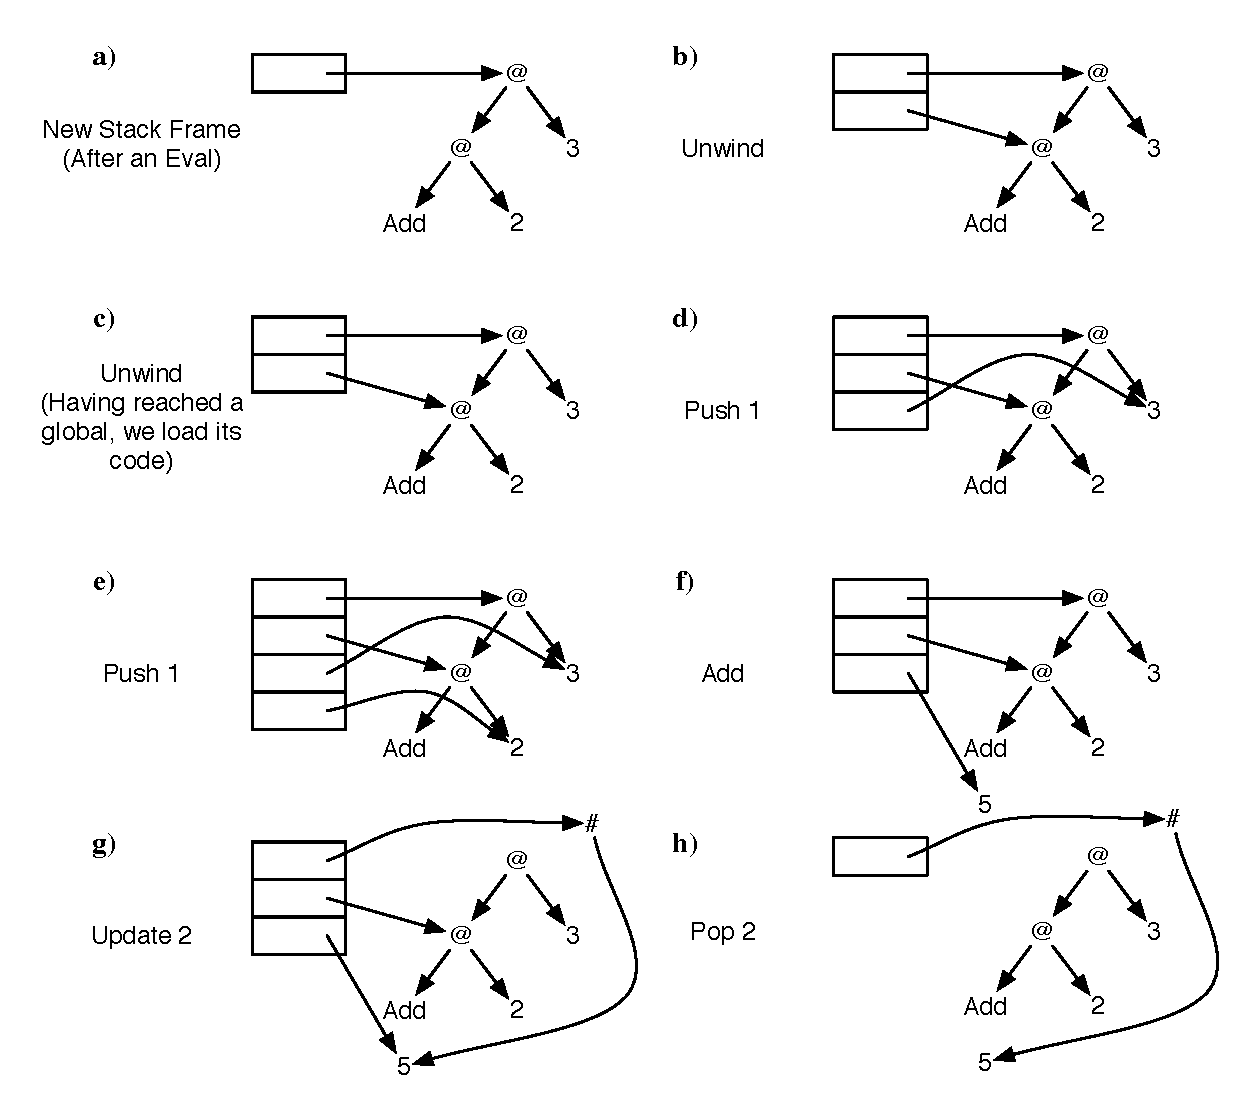
\includegraphics[scale=0.55]{Background/figures/AddExample.eps}
  \caption[G-Code execution example]
   {Walk-through of the \(G\)-Code for Add 2 3}
  \label{example:gCode}
\end{figure}

In figure \ref{example:gCode} we walk through a simple $G$-Machine reduction.
At (a) we have we have a reduction about to take place, the top of the stack is
pointing to the root of the expression. In (b) the GCode instruction Unwind is
executed, placing a pointer to the application node's function argument on the
stack. Unwinding continues until a global function is encountered.
When unwind reaches a global function, as in (c), the $G$-Machine loads
the code for that function and executes it. The code for \verb-Add- is Push 1,
Push 1, Add, Update 2, Pop 2, Unwind\footnote{This version of Add will only work
with primitives as its arguments. In order to accept expressions there would
need to be an Eval instruction added after every Push.}.
The first three instructions are what
actually add the two arguments, with the last three instructions being used to
update the graph and begin unwinding again. Push 1 pushes a pointer to the
argument of the application node pointed to by the address located at stack
address 1 (the stack addressing starts at 0). This is done twice at (d)
and (e) in order to have pointers to both arguments at the top of the stack.
Then we have the Add instruction which dereferences the top two pointers and
adds the resulting values, the resulting value is then pushed onto the stack;
this is seen at (f). With the result now on the stack, updating takes place, (g).
The Update instruction take a value (which is the arity of the function being
evaluated) and updates the stack pointer that originally pointed to the root of
the expression. The pointer is replaced by an indirection node, which is in turn
set to point to the same value as the top stack pointer. With the updating
finished the expression's original graph is no longer needed. Therefore, we can
pop all of the intermediate pointers on the stack, which will always be equal to
the arity of the expression. At (h) we are left with the updated pointer that
can now be used by the calling function. We execute the Unwind instruction again,
entering the $G$-Machine into its unwind state, which will ensure that the
proper stack jumping occurs when there is nothing left to evaluate (such as in
this case).

 \subsection{Spineless $G$-Machine}
    The standard $G$-Machine updates the shared graph after every reduction
step. While this is conceptually simple and easy to implement, such frequent
rewrites in the heap can be seen as wasteful. The Spineless
$G$-Machine improves on this by only updating the graph when loss of sharing is
a possibility \citep{burn1988spineless}. It is known as `spineless' because the
chain of application nodes that would make up the spine in the standard
$G$-Machine is not built up in the heap. Instead it is exclusively
accumulated on the stack until an update is required. The key point in this
variation of the $G$-Machine is that updating should be associated with the
potential loss of sharing and not with a reduction \citep{burn1988spineless}.

    The way this was accomplished was by adding a new type of application node
which they call a ``SAP'' node (for shared application). A SAP node indicates
that the node is `updatable' and that the result of any reduction at that node
should be updated in the graph.

    The mechanism for the updates is slightly different for functions than it is
for values. First let us look at how functions are handled. When a SAP node is
pushed onto the stack during an unwinding a new stack frame is created. When a
pointer outside of the bounds of the stack frame is required we can take this as
a signal that the reduction occurring at the updatable node has resulted in a
function that `fails' the arity test. We then rewrite the subgraph at the SAP
node since we know that sharing could be lost if we continued otherwise.
For values the update is triggered when the value has been reduced to its
base-value form.

    The remaining task for the Spineless $G$-Machine is to determine which
application nodes should be a SAP node, and which should be a standard AP node.
The authors give three different strategies for identifying which nodes should
be marked as SAP. The simplest strategy is that all nodes should be marked as
sharing nodes; this ensures that no sharing will be lost but will find the same
wasteful re-writing that the standard $G$-Machine exhibited. The next strategy
involves simple static sharing analysis to identify the nodes where the
arguments will definitely \emph{not} be shared, so all other nodes are marked as
sharing nodes. Lastly, a dynamic method is suggested that attempts to identify
as few sharing nodes as possible (therefore minimising the re-writing) while
adding an overhead cost of having to check when a shared subgraph is created.
The authors call this mechanism ``dashing'' and argue that the savings of having
as few re-writes as possible make the overhead cost of dashing worthwhile
\citep{burn1988spineless}.


 \subsection{STG-Machine}

A few years after the design of the Spineless $G$-Machine, another enhancement
was introduced, the Spineless Tagless $G$-Machine. This descendant of the
$G$-Machine is a fully realised Spineless $G$-Machine that eliminates the need
for tagged nodes by using a uniform representation for all value in its graph
representation. All values are represented on the heap as \emph{closures}.

Each closure consists of a code pointer and zero or more pointer fields used to
point to the values of free variables. The code the closure points to is what
determines the behavior of that node in the graph. When the code for a closure
is entered, the free variables can be access via an environment pointer that
points to the original node in the graph (which has the pointer fields
mentioned above) \citep{jones1992implementing}. Because there is no tag on a
node, the only way of determining the purpose of the node is to enter the
closure. As expressed by Peyton Jones ``each closure (including data values) is
represented uniformly, and scrutinized only by entering it.''
\citep{jones1992implementing}.

The STG-Machine uses the self-updating model when having to update a subgraph.
Instead of updating after every reduction, like the $G$-Machine, each closure
is responsible for updating itself when an update is necessary. In the case of
a thunk, entering the closure will result in the thunk being overwritten and
the resulting closure's code will simply return the value that has already been
evaluated.

The STG-Machine became the basis for GHC and has had many improvements over the
years \citep{HistoryOfHaskell}. Interestingly, one of the improvements to the
STG-Machine was the introduction of tags! The elegance of being able to treat
every node the same has a cost on the performance on modern architectures
\citep{marlow2007faster}.  Because so much of the performance in modern CPUs
comes from the speed of its cache (and therefore avoiding the memory
bottleneck) the indirections that arise from the code pointers in each closure
have a significant cost on performance. As stated in the introduction to their
2007 paper \citep{marlow2007faster}:

\begin{quote}
The tagless scheme is attractive because the code to evaluate a closure is
simple and uniform: any closure can be evaluated simply by
entering it. But this uniformity comes at the expense of performing indirect
jumps, one to enter the closure and another to return to
the evaluation site. These indirect jumps are particularly expensive
on a modern processor architecture, because they fox the branchprediction
hardware, leading to a stall of 10 or more cycles depending on the length of the
pipeline.
\end{quote}

As much as we would like to focus on elegant abstractions and distance
ourselves from any low level concerns, there will always be \emph{some} focus
on performance, and that will sometimes require compromises to accommodate
hardware realities.
